\section{Introduction}\label{sec:intro}

We will denote by $|a-b|_X$ the distance between points $a$ and $b$ in the metric space $X$.

\parbf{Tree comparison.}
Fix a tree $T$ with $n$ vertexes.

Let $(a_1,\dots a_n)$ be a point array in a metric space $X$ labeled by the vertexes of $T$.
We say that $(a_1,\dots a_n)$  satisfies the \emph{$T$-tree comparison} if there is a point array $(\~a_1,\dots, \~a_n)$ in the Hilbert space $\HH$ such that 
\[|\~a_i-\~a_j|_\HH\ge|a_i-a_j|_X\]
for any $i$ and $j$ and the equality holds if $a_i$ and $a_j$ are adjacent in $T$.

We say that a metric space $X$ satisfies the \emph{$T$-tree comparison} if 
every $n$-points array in $X$ satisfies the $T$-tree comparison.

Instead of the Hilbert space $\HH$ we may use infinite dimensional sphere or infinite dimensional hyperbolic space.
In this case we will it defines \emph{spherical} and \emph{hyperbolic} tree comparisons.

\hide
\begin{wrapfigure}{r}{27 mm}
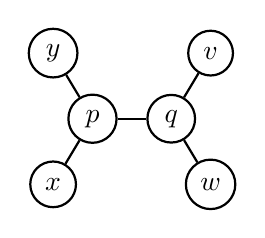
\begin{tikzpicture}[scale=1,
  thick,main node/.style={circle,draw,font=\sffamily\bfseries,minimum size=3mm}]
  \node[main node] (1) at (-1/2,-5/6) {$x$};
  \node[main node] (2) at (0,0){$p$};
  \node[main node] (3) at (-1/2,5/6){$y$};
  \node[main node] (4) at (3/2,5/6) {$v$};
  \node[main node] (5) at (1,0) {$q$};
  \node[main node] (6) at (3/2,-5/6) {$w$};

  \path[every node/.style={font=\sffamily\small}]
   (1) edge node[above]{}(2)
   (2) edge node[above]{}(3)
   (2) edge node[above]{}(5)
   (4) edge node[above]{}(5)
   (5) edge node[above]{}(6);
\end{tikzpicture}
\end{wrapfigure}
\unhide

\parbf{Encoding of trees.}
To encode the labeled tree on the diagram, we will use notation $p/xy(q/vw)$.
It means that we choose $p$ as the root; 
$p$ has two children leafs to $x$, $y$ and one child $q$ with two children leafs $v$ and $w$.
Taking another root for the same tree, we get different encodings, for eaxample $q/vw(p/xy)$ or $x/(p/y(q/vw))$.

If we do not need the labeling of vertexes,
it is sufficient to write the number of leafs in the brackets;
this way we can write 2(2) instead of $p/xy(q/vw)$ since the root ($p$) has 2 leafs ($x$ and $y$) and yet another child ($q$) which has 2 leafs ($v$ and $w$).  
The same tree can be encoded as (1(2)) meaning that the root $x$ has no leafs, 
$p$ has 1 leaf $y$ and one child $q$ with 2 leafs $v$ and $w$.
Every vertex which is not the root and not a leaf corresponds to a pair of brackets in this notation.

Using the described notation, we could say that a metric space \emph{satisfies the 2(2)-tree comparison},  meaning that it satisfies the tree comparison on the diagram.
We could also say \emph{``applying the $p/xy(q/vw)$-tree comparison...''} meaning that we apply the comparison for these 6 points labeled as on the diagram.

\parbf{Monopolar trees.}
A vertex of a tree of degree at least two will be called \emph{pole}.

\hide
\begin{wrapfigure}{r}{20 mm}
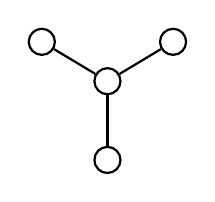
\begin{tikzpicture}[scale=1,
  thick,main node/.style={circle,draw,font=\sffamily\bfseries,minimum size=3mm}]

  \node[main node] (1) at (5/6,1) {};
  \node[main node] (2) at (0,3/2){};
  \node[main node] (3) at (10/6,3/2){};
  \node[main node] (4) at (5/6,0) {};

  \path[every node/.style={font=\sffamily\small}]
   (1) edge node[above]{}(2)
   (1) edge node[above]{}(3)
   (1) edge node[above]{}(4);
\end{tikzpicture}
\end{wrapfigure}
\unhide

Recall that \emph{Alexandrov space} with nonnegative curvature is defined as complete length space with curvature bounded below in the sense of Alexandrov;
the latter is equivalent to the 3-tree comparison; that is, the comparison for the tripod-tree on the diagram. 

Using the introduced notation, a theorem in \cite{AKP} can be restated the following way: \emph{If a complete length-metric space satisfies $3$-tree comparison, then it also satisfies $n$-tree comparison for every positive integer~$n$; in other words it satisfies all monopolar tree comparisons.}

\parbf{Bipolar trees.}
Consider the bipolar trees 3(1) and 2(2) shown on the diagram.

\hide
\begin{center}
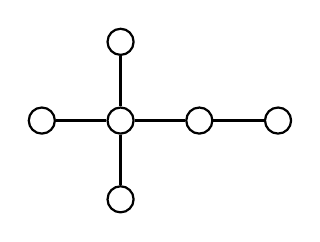
\begin{tikzpicture}[scale=1,
  thick,main node/.style={circle,draw,font=\sffamily\bfseries,minimum size=3mm}]

  \node[main node] (1) at (1,2) {};
  \node[main node] (2) at (1,0){};
  \node[main node] (3) at (1,1){};
  \node[main node] (4) at (0,1) {};
  \node[main node] (5) at (3,1) {};
  \node[main node] (6) at (2,1) {};

  \path[every node/.style={font=\sffamily\small}]
   (1) edge node[above]{}(3)
   (2) edge node[above]{}(3)
   (3) edge node[above]{}(6)
   (4) edge node[above]{}(3)
   (5) edge node[above]{}(6);
\end{tikzpicture}
\hskip30mm
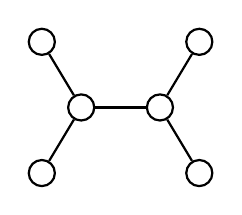
\begin{tikzpicture}[scale=1,
  thick,main node/.style={circle,draw,font=\sffamily\bfseries,minimum size=3mm}]

  \node[main node] (1) at (0,0) {};
  \node[main node] (2) at (1/2,5/6){};
  \node[main node] (3) at (0,10/6){};
  \node[main node] (4) at (2,0) {};
  \node[main node] (5) at (3/2,5/6) {};
  \node[main node] (6) at (2,10/6) {};

  \path[every node/.style={font=\sffamily\small}]
   (1) edge node[above]{}(2)
   (2) edge node[above]{}(3)
   (2) edge node[above]{}(5)
   (4) edge node[above]{}(5)
   (5) edge node[above]{}(6);
\end{tikzpicture}
\end{center}
\unhide
The following theorem states that the corresponding comparisons also follow form  Alexandrov's comparison.

\begin{thm}{Theorem}\label{thm:3(1)+2(2)}
Any Alexandrov space with nonnegative curvature satisfies  3(1)-tree and 2(2)-tree comparisons.
\end{thm}

\hide
\begin{wrapfigure}{r}{31 mm}
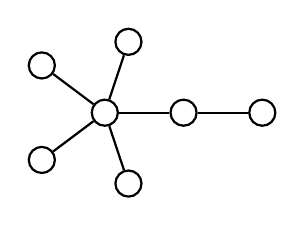
\begin{tikzpicture}[scale=1,
  thick,main node/.style={circle,draw,font=\sffamily\bfseries,minimum size=3mm}]

  \node[main node] (0) at (.3,.9){};
   \node[main node] (1) at (-.8,-.6){};
  \node[main node] (2) at (.3,-.9){};
  \node[main node] (3) at (0,0){};
  \node[main node] (4) at (-.8,.6){};
  \node[main node] (5) at (2,0){};
  \node[main node] (6) at (1,0){};

  \path[every node/.style={font=\sffamily\small}]
     (0) edge node[above]{}(3)
   (1) edge node[above]{}(3)
   (2) edge node[above]{}(3)
   (3) edge node[above]{}(6)
   (4) edge node[above]{}(3)
   (5) edge node[above]{}(6);
\end{tikzpicture}
\end{wrapfigure}
\unhide

The 4(1)-tree comparison turns out to be related to the  so called \emph{transport continuity property}, briefly TCP.
A compact Riemannian manifold $M$ is TCP 
if for any two regular measures with density functions bounded away from zero and infinity the generalized solution of Monge--Amp\`{e}re equation provided by optimal transport 
is a genuine solution.



A necessary condition for TCP was given by Xi-Nan Ma, Neil Trudinger and Xu-Jia Wang in \cite{MTW}.
A key step in the understanding this condition was made by Grégoire Loeper in~\cite{loeper}.
The manifolds satisfying this condition will be called \emph{cost-convex}.
We define it in the Section~\ref{sec:cost-convex}.

\begin{thm}{Theorem}\label{T=>CTIL:CTIL}
If a Riemannian manifold satisfies 4(1)-tree comparison then it is cost-convex; moreover it satisfies all bipolar tree comparisons.
\end{thm}

It is straightforward to check that the spherical 4(1)-tree comparison implies the strict cost-convexity, which in turns implies TCP; see \cite{FRV-Nec+Suf}.

The following question remains open.

\begin{thm}{Question}
Is it true that Rieamnnian manifold is cost-convex if and only if it satisfies 4(1)-tree comparison. 
\end{thm}

\parbf{All tree comparisons.}
Finally we consider spaces satisfying \emph{all tree comparisons}.

Recall that a map $f\:W\to X$ between metric spaces is called \emph{submetry} if for any $w\in W$ and $r\ge 0$, we have 
\[f[B(w,r)_W]=B(f(w),r)_X,\]
where $B(w,r)_W$ denotes the ball with center $w$ and radius $r$ in the space $W$.
In other words submetry is a map which is 1-Lipschitz and 1-co-Lipschitz at the same time.
Note that by the definition, any submetry is onto.

\begin{thm}{Theorem}\label{thm:hilbert-quotient}
A separable metric space $X$ satisfies all tree comparisons if and only if
$X$ is isometric to a target space of submetry defined on a subset  of the Hilbert space.
\end{thm}

The following proposition provides a source of examples of spaces satisfying all tree comparisons.
For example, since $\SS^n=\SO(n)/\SO(n-1)$, any round sphere has this property.


\begin{thm}{Proposition}\label{prop:group}
Suppose $G$ is a compact Lie group with bi-invariant metric, so the action $G\times G\acts G$ defined by $(h_1,h_2)\cdot g=h_1\cdot g\cdot  h_2^{-1}$ is isometric. 
Then for any closed subgroup $H<G\times G$, the bi-quotient space $G/\!\!/H$ satisfies all tree comparisons
\end{thm}

From proposition above and Theorem~\ref{T=>CTIL:CTIL}, it follows that the bi-quotient space $G/\!\!/H$ is cost-convex and  equivalently CTIL and MTW, see Section~\ref{sec:cost-convex}.
This makes it closely related to the result of Young-Heon Kim and Robert McCann in \cite{kim-mccann}.

\section{Digressions}

\parbf{On matrix inequality.}
The comparison for monopolar trees has an algebraic corollary which was first used Urs Lang and Viktor Schroeder in \cite{LS} and latter rediscovered by Karl-Theodor Sturm in \cite{sturm}. 
Namely, given a point array $p,x_1,\dots,x_n$ in a metric space $X$ consider the matrix $M$ with the components 
\[m_{i,j}=\tfrac12\cdot(|x_i-p|^2+|x_j-p|^2-|x_i-x_j|^2).\]
If $p/x_1,\dots,x_n$-tree comparison holds then 
\[\bm{s}\cdot M\cdot \bm{s}^\top\ge 0\]
for any vector $\bm{s}=(s_1,\dots,s_n)$ with nonnegative components.

\hide
\begin{wrapfigure}[7]{r}{22 mm}
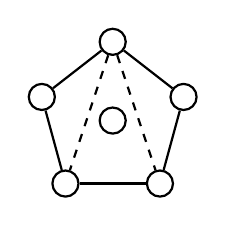
\begin{tikzpicture}[scale=1,
  thick,main node/.style={circle,draw,font=\sffamily\bfseries,minimum size=3mm}]

    \node[main node] (0) at (0,0){};
     \node[main node] (1) at (.6,-.8) {};
     \node[main node] (2) at (.9,.3){};
     \node[main node] (3) at (0,1) {};
  \node[main node] (4) at (-.9,.3) {};
  \node[main node] (5) at (-.6,-.8) {};

  \path[every node/.style={font=\sffamily\small}]
  (1) edge node[above]{}(2)
  (2) edge node[above]{}(3)
  (3) edge node[above]{}(4)
  (4) edge node[above]{}(5)
  (5) edge node[above]{}(1)
  (3) edge[dashed] node[above]{}(1)
   (3) edge[dashed] node[above]{}(5);
\end{tikzpicture}
\end{wrapfigure}

However, this condition is not sufficient for $p/x_1,\dots,x_n$-tree comparison with $n\ge 5$.
(In general, is not easy to describe tree comparisons using a system of inequalities.)

An example can be constructed by perturbing the configuration on the plane as on the diagram ---
if the diameter of diagram is 1, 
then increasing the distances between the pairs of points connected by dashed lines by $\eps=10^{-9}$ and decreasing  the distances between the pairs of points connected by sold lines by $\delta=10^{-6}$ does the job.
The obtained metric 6-point metric space satisfies the matrix inequality with center at each point, but does not satisfy the tree comparison with pole at the central point.


\parbf{On graph comparison.}
Analogously to the tree comparison one can define graph comparison for any graph by stating that there is model configuration such that the distance between pairs of adjacent points is at most as big and nonadjacent is at least as big.

\begin{thm}{Exercise}
Show that if a graph is a tree then the graph comparison defined above is equivalent to the tree comparison defined at the beginning of the paper.
\end{thm}


Note that nonnegative and nonpositive curvature can be defined using the comparison for following two graphs on 4 vertexes:

\hide
\begin{center}
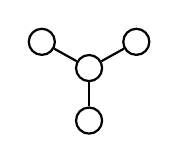
\begin{tikzpicture}[scale=1,
  thick,main node/.style={circle,draw,font=\sffamily\bfseries,minimum size=3mm}]

  \node[main node] (0) at (0,0) {};
  \node[main node] (1) at (-3/5,1/3){};
  \node[main node] (2) at (3/5,1/3){};
  \node[main node] (3) at (0,-2/3) {};

  \path[every node/.style={font=\sffamily\small}]
   (0) edge node[above]{}(1)
   (0) edge node[above]{}(2)
   (0) edge node[above]{}(3);
\end{tikzpicture}
\hskip30mm
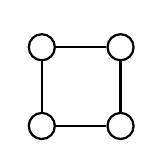
\begin{tikzpicture}[scale=1,
  thick,main node/.style={circle,draw,font=\sffamily\bfseries,minimum size=3mm}]

  \node[main node] (1) at (0,0) {};
  \node[main node] (2) at (0,1){};
  \node[main node] (3) at (1,1){};
  \node[main node] (4) at (1,0) {};

  \path[every node/.style={font=\sffamily\small}]
   (1) edge node[above]{}(2)
   (1) edge node[above]{}(4)
   (2) edge node[above]{}(3)
   (3) edge node[above]{}(4);
\end{tikzpicture}
\end{center}
\unhide

By Reshetnyak majorization theorem,
the nonpositive curvature could be also defined using the comparison for cycle; for example the 6-cycle, the first graph the following diagram.

\hide
\begin{center}
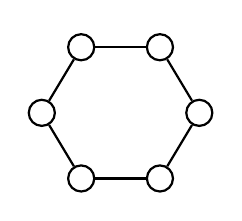
\begin{tikzpicture}[scale=1,
  thick,main node/.style={circle,draw,font=\sffamily\bfseries,minimum size=3mm}]

  \node[main node] (4) at (3/2,5/6){};
   \node[main node] (1) at (1/2,-5/6){};
  \node[main node] (2) at (3/2,-5/6){};
  \node[main node] (0) at (0,0){};
  \node[main node] (5) at (1/2,5/6){};
  \node[main node] (3) at (2,0){};


  \path[every node/.style={font=\sffamily\small}]
    (0) edge node[above]{}(1)
   (1) edge node[above]{}(2)
    (2) edge node[above]{}(3)
   (3) edge node[above]{}(4)
   (4) edge node[above]{}(5)
   (5) edge node[above]{}(0);
\end{tikzpicture}
\hskip30mm
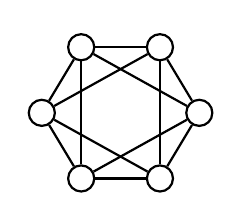
\begin{tikzpicture}[scale=1,
  thick,main node/.style={circle,draw,font=\sffamily\bfseries,minimum size=3mm}]

  \node[main node] (4) at (3/2,5/6){};
   \node[main node] (1) at (1/2,-5/6){};
  \node[main node] (2) at (3/2,-5/6){};
  \node[main node] (0) at (0,0){};
  \node[main node] (5) at (1/2,5/6){};
  \node[main node] (3) at (2,0){};


  \path[every node/.style={font=\sffamily\small}]
    (0) edge node[above]{}(1)
   (1) edge node[above]{}(2)
    (2) edge node[above]{}(3)
   (3) edge node[above]{}(4)
   (4) edge node[above]{}(5)
   (5) edge node[above]{}(0)
    (0) edge node[above]{}(2)
   (1) edge node[above]{}(3)
    (2) edge node[above]{}(4)
   (3) edge node[above]{}(5)
   (4) edge node[above]{}(0)
   (5) edge node[above]{}(1);
\end{tikzpicture}
\end{center}
\unhide

The comparison for the second graph implies that the space is nonnegatively curved.
The latter follows since in this graph, a 4-cycle appears as an induced subgraph.
On the other hand, this comparison might be stronger and it might be interesting to understand.

(The tree comparison holds for factors spaces of Hilbert space --- this was the main motivation to consider this type of comparison. 
Unfortunately we do not have analogous examples of nonnegatively curved spaces which would guide us to the right definition.)

\parbf{On colored graph comparison.}
It is also possible to use graph with $(\mp)$-colored edges and define comparison by model configuration such that the distances between vertexes adjacent by a $(-)$-edge does not get larger and by $(+)$-edge does not get smaller.
For example, the $(2{\cdot}n+2)$-comparison (which holds in $\CAT[0]$ length spaces, see \cite{AKP}) can be considered as a comparison for the following colored graph, where $(-)$-edges are marked by solid lines and $(+)$-edges by dashed lines.

\hide
\begin{center}
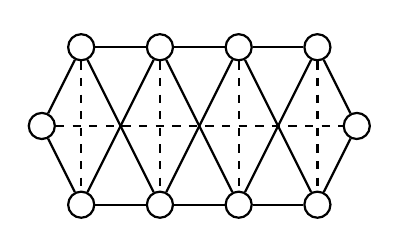
\begin{tikzpicture}[scale=1,
  thick,main node/.style={circle,draw,font=\sffamily\bfseries,minimum size=3mm}]

  \node[main node] (0) at (0.5,0){};
   \node[main node] (1) at (1,1){};
  \node[main node] (2) at (1,-1){};
  \node[main node] (3) at (2,1){};
  \node[main node] (4) at (2,-1){};
  \node[main node] (5) at (3,1){};
\node[main node] (6) at (3,-1){};
 \node[main node] (7) at (4,1){};
\node[main node] (8) at (4,-1){};
\node[main node] (100) at (4.5,0){};

  \path[every node/.style={font=\sffamily\small}]
    (0) edge[dashed] node[above]{}(100)
   (1) edge[dashed] node[above]{}(2)
    (3) edge[dashed] node[above]{}(4)
   (5) edge[dashed] node[above]{}(6)
   (7) edge[dashed] node[above]{}(8)
   (0) edge node[above]{}(1)
   (0) edge node[above]{}(2)
    (1) edge node[above]{}(3)
   (2) edge node[above]{}(4)
   (1) edge node[above]{}(4)
   (2) edge node[above]{}(3)
   (5) edge node[above]{}(3)
   (6) edge node[above]{}(4)
   (5) edge node[above]{}(4)
   (6) edge node[above]{}(3)
   (5) edge node[above]{}(7)
   (6) edge node[above]{}(8)
   (5) edge node[above]{}(8)
   (6) edge node[above]{}(7)
   (7) edge node[above]{}(100)
   (8) edge node[above]{}(100);
\end{tikzpicture}
\end{center}
\unhide